\section{Paragraf autorstwa Jana Majchrowicza}
Wzmacniacz sumujący jest aplikacją wzmacniacza operacyjnego, która służy do złączenia dwóch (lub więcej) napięć wejściowych w jedno i wyprowadzeniu go na wyjście wzmacniacza.
\\
\\
    \LARGE{\textbf{Układ wzmacniacza sumującego}}
\subsection{Podstawowe wzory:}
        \begin{figure}[htbp]
            \centering
            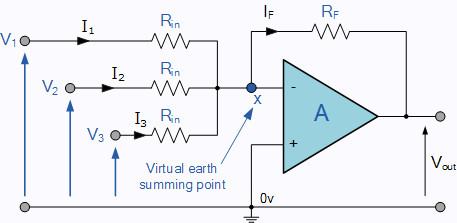
\includegraphics[width=1\textwidth]{pictures/wzmacniacz1.jpg}
            \caption{\textbf {WZMACNIACZ SUMUJĄCY}}
            \label{fig:wzmacniacz}
        \end{figure}
\large{W tym prostym układzie wzmacniacza sumującego, napięcie wyjściowe $V_{OUT}$ jest proporcjonalne do sumy napięć wejściowych: $V_{1}$, $V_{2}$, $V_{3}$ itd. Możemy zmodyfikować oryginalne równanie dla wzmacniacza odwracającego, aby uwzględnić te nowe wejścia, w następujący sposób:}
\\
\\
    \begin{equation} \label{eq:1}
        I_{f}=I_{1}+I_{2}+I_{3}=-\left[\frac{V_{1}}{R_{IN}}+\frac{V_{1}}{R_{IN}}+\frac{V_{1}}{R_{IN}}\right]
    \end{equation}
    \\
    \\
Wynika z tego:
    \begin{equation} \label{eq:1}
        V_{OUT}=-\frac{R_{F}}{R_{in}} \times V_{in}
    \end{equation}
\\
Po przekształceniu:
    \begin{equation} \label{eq:1}
        V_{OUT}=-\left[\frac{R_{F}}{R_{in}}V_{1} + \frac{R_{F}}{R_{in}}V_{2}+\frac{R_{F}}{R_{in}}V_{3}\right]
    \end{equation}
    
\large{Mamy układ ze wzmacniaczem operacyjnym, który wzmacnia każde napięcie wejściowe i wytwarza napięcia wyjściowego, które jest proporcjonalne do algebraicznej sumy trzech poszczególnych napięć wejściowych: $V_{1}$, $V_{2}$ i $V_{3}$. Można dodać więcej wejść, jeśli jest to wymagane, ponieważ każde wejście „widzi” swoją odpowiednią rezystancję, $R_{in}$. Wynika to z faktu, że sygnały wejściowe są skutecznie odizolowane od siebie przez węzeł „wirtualnej masy” na wejściu odwracającym wzmacniacza operacyjnego, czyli nie przenikają między sobą. Dodawanie napięć bez wzmacniania można również uzyskać, gdy wszystkie rezystancje są równej wartości, a $R_{F}$ jest równe $R_{in}$. Jedynie wynikowa suma będzie odwrócona w fazie o $180^\circ$, co wynika z odwracającego charakteru układu.}
\\
\\
\subsection{Przykładowe aplikacje wzmacniacza operacyjnego:}
\begin{itemize}
  \item Wzmacniacz odwracający
  \item Wzmacniacz nieodwracający
  \item Wzmacniacz sumujący (rysunek \ref{fig:wzmacniacz})
  \item Wzmacniacz odejmujący
  \item Wzmacniacz całkujący
  \item Wzmacniacz różniczkujący
\end{itemize}

\subsection{Niektóre zastosowania wzmacniaczy operacyjnych:}
\begin{enumerate}
    \item Układy dopasowujące
    \item Układy filtrujące
    \item Układy wykonujące skomplikowane operacje matematyczne
    \item Generatory
    \item Wtórniki
    \item Prostowniki
\end{enumerate}
I inne...
\\
\\
Do powyższych układów można użyć modeli wzmacniaczy z tabeli na stronie \pageref{tab:tabelka}
\\
\\

\subsection{Niektóre modele wzmacniaczy operacyjnych}

\begin{table}[htbp]
\label{tab:tabelka}
\begin{tabular}{|c|c|c|}
\hline
Symbol & Nazwa                   & Opis                    \\ \hline
AD830  & Układ scalony AD830AN   & Single High-Speed Video \\ \hline
HA5002 & Układ scalony HA3-5002  & SINGLE WIDEBAND         \\ \hline
LM358  & Układ scalony LM358     & DUAL Low Power          \\ \hline
LM392  & Układ scalony LM392     & Komparator + Wzmacniacz \\ \hline
TL071  & Układ scalony TL071 Pbf & SINGLE J-FET            \\ \hline
\end{tabular}
\end{table}